\begin{frame}
\frametitle{Task 5: Theory}
Consider now the spherical coordinates 
\begin{equation}
\hat{r} = sin\theta cos\phi \hat{x} + sin\theta sin\phi \hat{y} + cos\theta \hat{z},
\end{equation}

\begin{align}
& d_n = \mathbf{r}_n \cdot \hat{r} = (x_n\hat{x}+ y_n\hat{y} + z_n\hat{z}) (sin\theta cos\phi \hat{x} + sin\theta sin\phi \hat{y} + cos\theta \hat{z})= \\
& sin\theta_0 cos\phi_0 x_n + sin\theta_0 sin\phi_0 y_n + cos\theta_0 z_n.
\end{align}

\begin{equation}
\Psi_{n, 0} = kd_{n,0} = \frac{2\pi}{\lambda} | sin\theta_0 cos\phi_0 (x_n) + sin\theta_0 sin\phi_0 (y_n)  + cos\theta_0 (z_n)|. 
\end{equation}

Amplitude of current was set to 1 A
\end{frame}



\begin{frame}
\frametitle{Task 5: Results}
\begin{columns}[c]
\column{.45\textwidth}
\begin{figure}[h]
\centering
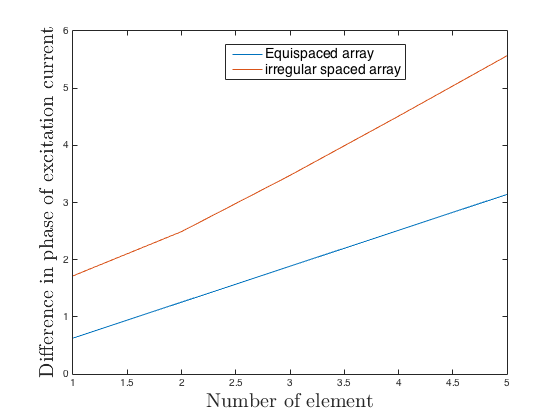
\includegraphics[scale=0.3]{/Users/marikasvensson/Documents/MATLAB/MicroProject/finished/task5/excitationCurrent.png}
\caption{This figure shows the phase of the excitation current as a function of element positions and steering direction $\theta_0 = \pi/3$rad and $\phi_0 = \pi/2$rad }
\label{task5:phase}
\end{figure}

\column{.5\textwidth} 
\begin{figure}[h]
\centering
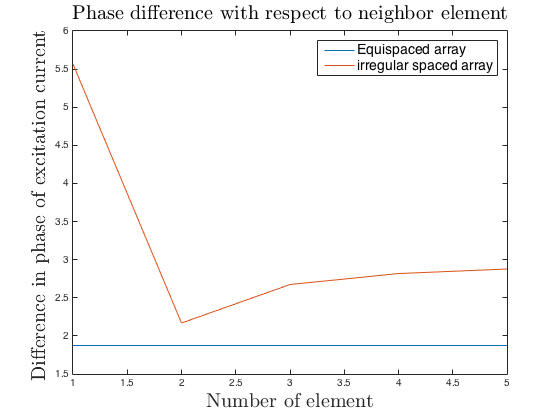
\includegraphics[scale=0.3]{/Users/marikasvensson/Documents/MATLAB/MicroProject/finished/task5/excitationCurrentNeighbour.png}
\caption{This figure shows the phase of the excitation current with respect to the neighbor as a function of element positions and steering direction $\theta_0 = \pi/3$rad and $\phi_0 = \pi/2$rad }
\label{task5:phaseNeigh}
\end{figure}
\end{columns}
\end{frame}

